\section{非代数闭域上的约态概形}

现在我们考虑当观察非代数闭域上的有限生成约态代数\index{约态!代数}的谱时将会发生什么。对这样的结构的兴趣最早来自于数论,当然,它远比概形理论要早得多!比如,关于有理二次型的研究,这是数论中一个古老的课题,能看作对有理数域上二次方程定义的簇的研究。研究有理数域上三个变量的三次型在数论上至今依然是非常活跃的方向,其中现在主要醉心于$\mathbb{Q}$上的椭圆曲线理论。虽然这里最基本的对象是$\mathbb{Q}$上的代数簇(或是$\mathbb{Z}$上的概形,我们以后会回到这个情况),但在处理它们的过程中,数论学家常常使用下面这副图中这些所有的基环,以及许多的中间域以及中间环:
\[
\begin{xy}
	\xymatrix{
		\hat{\mathbb{Z}}_{(p)}\ar[r]&\hat{\mathbb{Q}}_{p}\ar[rr]&&\mathbb{C}_p\\
		\mathbb{Z}_{(p)}\ar[u]&&&\\
		\mathbb{Z}\ar[u]\ar[r]\ar[d]&\mathbb{Q}\ar[r]\ar[uu]&\mathbb{R}\ar[r]&\mathbb{C}\ar[uu]\\
		\mathbb{F}_p\ar[r]&\bar{\mathbb{F}}_p&&&
	}
\end{xy}
\]
概形理论提供了一个相当富有弹性且舒适的框架来处理这些基环的改变。此外,一个性质良好的约态簇,在模$p$后可能突然变成一个非约态的东西,描述这东西需要更完整的概形理论(比如见\ref{sec:2.4.4}节)。

从最简单的例子开始,考虑$\mathbb{A}_{\mathbb{R}}^1=\spec \mathbb{R}[x]$. 使用Nullstellensatz,可以看到$R[x]$中有两类极大理想:一类的剩余类域是$\mathbb{R}$,它们具有形式$(x-\lambda)$,其中$\lambda\in\mathbb{R}$,剩余类域是$\mathbb{C}$,它们具有形式$(x^2+\mu x+\nu)$,其中$\mu$, $\nu\in\mathbb{R}$且满足$\mu^2-4\nu<0$. 另一类理想可以写作$((x-z)(x-\bar{z}))$的形式,其中$z\in \mathbb{C}$不是一个实数。于是,$\mathbb{A}_{\mathbb{R}}^1$中的闭点,对应于一个实数或者一对共轭的复数。最后,$\mathbb{A}_{\mathbb{R}}^1$同样有着唯一的非闭点,对应于素理想$(0)$,它的闭包是整个$\mathbb{A}_{\mathbb{R}}^1$.

接着,我们来到$\mathbb{R}$上的仿射平面,$\mathbb{A}_{\mathbb{R}}^2=\spec \mathbb{R}[x,y]$,以及考虑$R[x,y]$的极大理想$\mathfrak{m}$给出的闭点。同样从Nullstellensatz,$R[x,y]$关于$\mathfrak{m}$的剩余类域只有$\mathbb{R}$与$\mathbb{C}$,于是复合映射
\[
	\rr\to \rr[x,y]/\mm\cong (\rr \text{ or } \cc)
\]
或者是恒同或者是$\rr$到$\cc$的含入。取$\lambda$和$\mu$作为$x$和$y$在$\cc$中的像,对前一种情况,我们可以看到$\mm=(x-\lambda,y-\mu)$对应于$\rr^2$中一般意义上的点。但是对后一种情况,$\mm$同时对应于$(\lambda,\mu)$和$(\bar\lambda,\bar\mu)$:从另一种视角来看,将$x$, $y$变成$\lambda$, $\mu$的同态$\rr[x,y]\to \cc$与另一个将$x$, $y$变成$\bar\lambda$, $\bar\mu$的同态有着相同的核,因为它们只差一个$\cc$在$\rr$上的自同构。

给出上面描述的极大理想的生成元并不是件很困难的事情。如果$\rr[x,y]/\mm\cong \rr $,很清楚地,$\mm=(x-\lambda,y-\mu)$. 另一方面,假设$\lambda$是实数,则$\mu$必须要满足一个不可约二次实系数多项式$y^2+ay+b=0$,于是$\mm$包含理想$(x-\lambda,y^2+ay+b)$. 但这个理想显然是一个素理想(比如,先模掉$x-\lambda$因子),于是$\mm=(x-\lambda,y^2+ay+b)$. 自然,当$\mu$是实数的时候,类似的结果也成立。

最后,假设$\mu$和$\lambda$都不是实数,于是$\mm$包含以$\mu$和$\lambda$为根的不可约实系数多项式$f$和$g$,但是,因为$g$可以在$\rr[x]/(f(x))\cong \cc$上分解为
\[
	g(y)=(y-\mu)(y-\bar\mu),
\]
因此$(f(x),g(y))$不是素理想!在复数域上,可以给出如下图像:

\begin{center}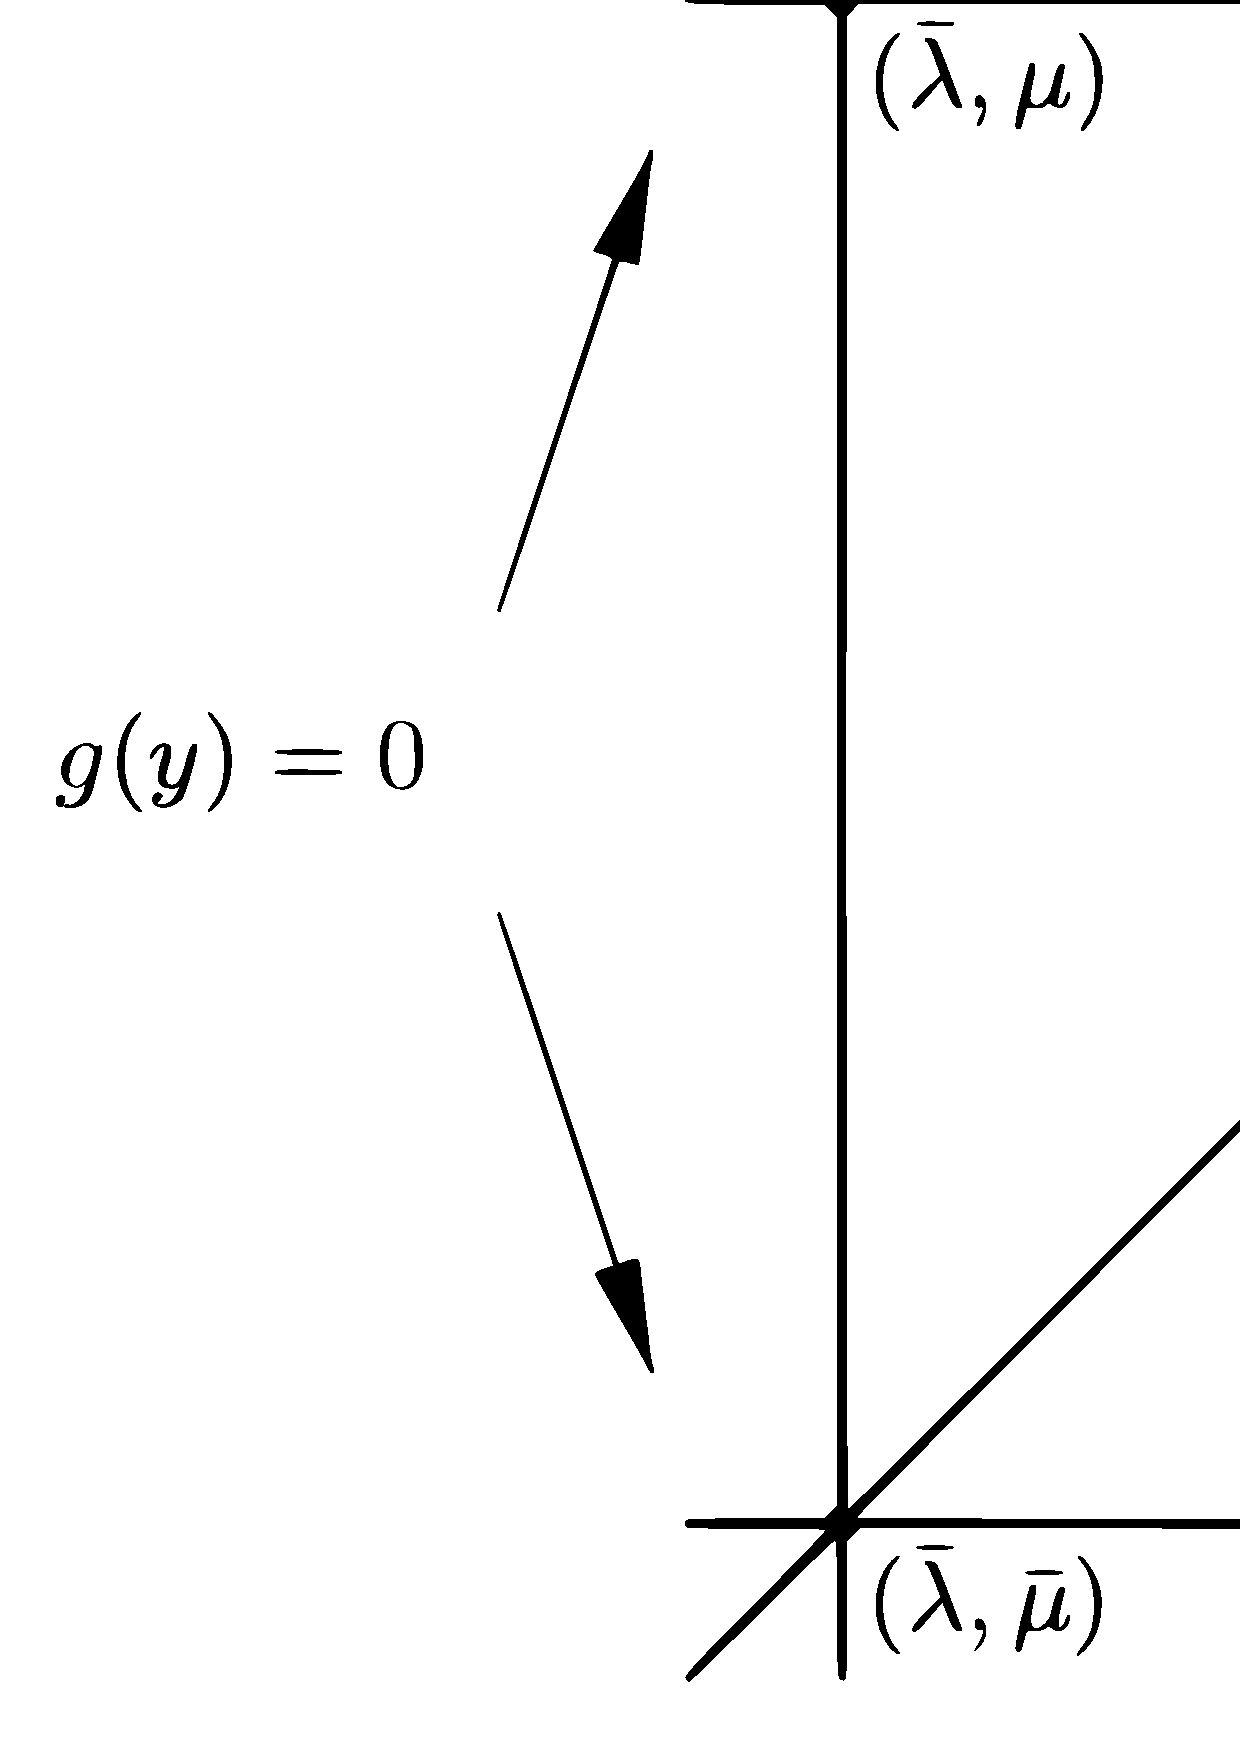
\includegraphics[scale=\scale,bb=0 0 683 419]{chap_2/pics/5.png}\end{center}

$f(x)=0$与$g(y)=0$的零点集分别是两条水平线与数值线的并,它们相交于四点$(\lambda,\mu)$, $(\bar\lambda,\mu)$, $(\lambda,\bar\mu)$和$(\bar\lambda,\bar\mu)$. 多项式
\[
	h(x,y)=\mathrm{Im}(\mu) x - \mathrm{Im}(\lambda)  y -\mathrm{Im}(\mu\bar\lambda)
\]
是连接$(\lambda,\mu)$和$(\bar\lambda,\bar\mu)$的那条实系数直线。理想
\[
	(f(x),h(x,y))=(g(y),h(x,y))\subset \rr[x,y]
\]
严格包含理想$(f(x),g(y))$,它就是我们寻找的极大理想,这点可以通过检查
\[
	\rr[x]\cong \rr[x,y]/(h)\cong \rr[y]
\]
得到(这些同构中,注意到$(\bar\mu-\mu)$与$(\bar\lambda-\lambda)$都非零)。

总之,$\mathbb{A}_{\rr}^2$的闭点集,对应于$\mathbb{A}_{\cc}^2$中的点$(\lambda,\mu)$,其中$\lambda$和$\mu$都是实数,或者对应于(无序)偶对$(z,w)$或者$(\bar z,\bar w)\in \mathbb{A}_{\cc}^2$,其中$z$, $w$至少有一个不是实数。从另一种角度来看,$\mathbb{A}_{\rr}^2$的闭点对应于$\mathbb{A}_{\cc}^2$中点共轭作用后的轨道。(注意,特别地,$\mathbb{A}_{\rr}^2$的闭点不是$\mathbb{A}_{\rr}^1$中闭点的有序偶对!)同样可以注意到,$\mathbb{A}_{\rr}^2$中点$(\lambda,\mu)$处的剩余类域是$\rr$,其中$\lambda$, $\mu$都是实数,而$\mathbb{A}_{\rr}^2$中复共轭的一对点处的剩余类域是$\cc$.

\begin{exe}
	证明$\mathbb{A}^2_{\rr}$的全部非闭点是
	\begin{compactenum}[(a)]
		\item $[(0)]$,它的闭包是整个$\mathbb{A}^2_{\rr}$,或者
		\item 点$[(f)]\in \mathbb{A}^2_{\rr}$对应于不可约多项式$f\in \rr[x,y]$.
	\end{compactenum}

	上面的(b)类点的多项式在$\cc[x,y]$中不一定还是不可约的,故$\mathbb{A}^2_{\rr}$中的非闭点$(f)$会对应于$\mathbb{A}^2_{\cc}$的一个非闭点($f$在$\cc[x,y]$中还是不可约的)或者两个非闭点($f$在$\cc[x,y]$能写成乘积$g\bar g$,其中$g\in\cc[x,y]$). 这样的非闭点的闭包中的闭点,要么上面的第一类第二类都有,要么只有第二类。试给出所有这些可能性的例子。
\end{exe}

一般的情况按下面这列例子进行:如果$K$是任意的域,$\bar K$是它的代数闭包,而$G=\mathrm{Gal}(\bar K/K)$是对应的Galois群,则$\mathbb{A}_{K}^n$中的点对应于$G$作用在$\mathbb{A}_{\bar K}^n$上的点的轨道(比如见Nagata [1962, Theorem 10.3])。闭点对应于闭点的轨道,而轨道是有限的。点$p$处的剩余类域,对应于在某条轨道上使其一点不动的子群$G_p$作用在$\bar K$上的不变域。比如,$\mathbb{A}^1_\mathbb{Q}$的闭点对应于代数数模掉共轭;以及对素数$q\in \mathbb{Z}$,$\mathbb{A}_{\mathbb{F}_q}^1$的闭点对应于$\mathbb{F}_q=\mathbb{Z}/(q)$的代数闭包的Frobenius自同构的轨道(即,$0$以及映射$a\mapsto a^q$在乘法群$\bar K^*$上的轨道,也能被描述为所有阶数与$q$互素的循环群的归纳极限,或者是$\mathbb{Q}/\mathbb{Z}$的$q$-无挠部分)。

\begin{exe}
	域的含入映射$K\hookrightarrow L$诱导了映射$\mathbb{A}_L^n\to \mathbb{A}_K^n$. 找出下面这些$\mathbb{A}_{\overline{\mathbb{Q}}}^n$的点在这个映射下在$\mathbb{A}_{\mathbb{Q}}^n$中的像。
	\begin{compactenum}[(a)]
		\item $(x-\sqrt{2},y-\sqrt{2})$
		\item $(x-\sqrt{2},y-\sqrt{3})$
		\item $(x-\zeta,y-\zeta^{-1})$,其中$\zeta$是$p$次单位根,而$p$是一个素数
		\item $(\sqrt{2}x-\sqrt{3}y)$
		\item $(\sqrt{2}x-\sqrt{3}y-1)$
	\end{compactenum}
	如果可能则做出图像。
\end{exe}

\begin{exe}
	我们说子概形$X\subset \mathbb{A}_K^n$是\textit{绝对不可约的}\index{不可约!绝对}或者是\textit{几何不可约的}如果$X$在$\mathbb{A}_{\bar K}^n$中的原像是不可约的。(更一般地,我们说任意$K$\hyp 概形$X$是绝对不可约的如果纤维积$X\times_{\spec K}\spec \bar{K}$是不可约的。)将下面这些$\mathbb{A}_\mathbb{Q}^2=\spec \mathbb{Q}[x,y]$的子概形分类成可约的、不可约但不是绝对不可约的或者绝对不可约的。
	\begin{compactenum}[(a)]
		\item $V(x^2-y^2)$
		\item $V(x^2+y^2)$
		\item $V(x^2+y^2+1)$
		\item $V(x+y,xy-2)$
		\item $V(x^2-2y^2,x^3+3y^3)$
	\end{compactenum}
\end{exe}

最后,这里有一个联合了局部概形与非代数闭域上的概形两个概念的例子。经典地,对平面曲线$X\subset \mathbb{A}_\cc^2$,如果在原点处有一个解析邻域,使得在其中$Y$的复点的轨迹\footnote{译者注:原文是``if in some analytic neighborhood of the origin the locus of complex points of $Y$''. $Y$似乎应该理解成$X$在这个解析邻域里面的像。复点的意思在后文才被揭示,是在那里剩余类域为$\cc$的点。 ``locus''请允许我翻译成轨迹,其实想象成这些点的集合就行,毕竟是经典图像。}$Y$由两条在$(0,0)$处横截相交的光滑弧构成,则$X$被称为在原点处有一个\idx{结点}(node)。在概形的语言中,这等价于说,$X$与形式邻域$\spec \cc[\![x,y]\!]\to \spec \cc[x,y]=\mathbb{A}_\cc^2$的纤维积同构于$\spec \cc[\![u,v]\!]/(uv)$.

现在考虑实平面上的曲线$X\subset \mathbb{A}_\rr^2$. 这种情况下,我们称$X$在原点处有一个结点,如果对应的复曲线
\[
	X\times_{\spec \rr}\spec \cc \subset \mathbb{A}_\cc^2
\]
在原点处有。在这个例子里,形式邻域
\[
	X\times_{\spec \rr[x,y]}\spec \rr[\![x,y]\!]
\]
可能具有两种形式,同构于$\spec \rr[\![u,v]\!]/(uv)$或同构于$\spec \rr[\![u,v]\!]/(u^2+v^2)$,这两种形式不同构。前一种情况是如果$X$的实点的轨迹(即剩余类域为$\rr$的点的轨迹)在$(0,0)$的解析邻域中看上去像是两条光滑实弧线横截相交,经典地,这样的点被称为$X$的\idx{叉点}(acrunode)。后一种情况是原点作为$X$的实点被孤立了,这样点以前被称为\idx{孤立点}(acnode)。

\begin{exe}
	验证上面的断言:明确来说,证明如果$\mathbb{A}_\cc^2$中的曲线$X$在原点处有一个结点,则形式邻域$X\times_{\spec \cc[x,y]}\spec \cc[\![x,y]\!]$同构于$\spec\cc[\![x,y]\!]/(uv)$;以及,如果$X\subset \mathbb{A}_{\rr}^2$是一个在原点处有结点的实曲线,那么形式邻域$X\times_{\spec \rr[x,y]}\spec \rr[\![x,y]\!]$是上面提到的两种形式中的一个。证明,存在无限多在原点有结点的曲线$X\subset \mathbb{A}_{\mathbb{Q}}^2$有着不同构的形式邻域。(正如实数情况,我们称$X\subset \mathbb{A}^2_\mathbb{Q}$在原点处有结点,如果对应的复曲线$X\times_{\spec \mathbb{Q}} \spec \cc$有。)
\end{exe}